\documentclass{article}

% these packages let you do math
\usepackage{amsmath}
\usepackage{amssymb}

% we need these packages for fancy R tables
\usepackage{booktabs}
\usepackage{float}
\usepackage{colortbl}
\usepackage{xcolor}

% these packages play with the spacing/margins of the document. Uncomment the commands on lines 16 and 17 to see what they do.
\usepackage{a4wide}
\usepackage{setspace}
\usepackage{geometry}
\usepackage{parskip}
%\doublespacing
%\geometry{margin=1.5in}

% this package helps us with including images. Setting the graphics path makes it easier to refer to things in the \includegraphics command.
\usepackage{graphicx}
\graphicspath{ {../figures/} }

% make some hyperlinks using the \href command
\usepackage{hyperref}
\hypersetup{
    colorlinks=true,
    linkcolor=black,
    urlcolor=blue
}

% set the author, title, and date of the document. \maketitle adds it to the document.
\author{Xiaohan Wu}
\title{Paper on NLSY97 Data of Incarceration Status}
\date{Spring 2022}

\begin{document}
\maketitle

\section{Introduction}

This report describes patterns in incarceration status by race and gender in the year 2002, using NLSY97 publicly available data. Before analyzing the dataset, the raw dataset was mined into a clean dataset with readable variables wanted.

The three variables to be analyzed are \texttt{race}, \texttt{gender}, and \texttt{total\_incarcerated}. The variable \texttt{race} includes \texttt{Black}, \texttt{Hispanic}, \texttt{Mixed Race}, and \texttt{Non-Black or Non-Hispanic}. The variable \texttt{total\_incarcerated} represents the count of months of incacerations in 2022 for the respondent who has the crime record.

\section{Analysis}

\begin{figure}[H]
    \begin{center}
        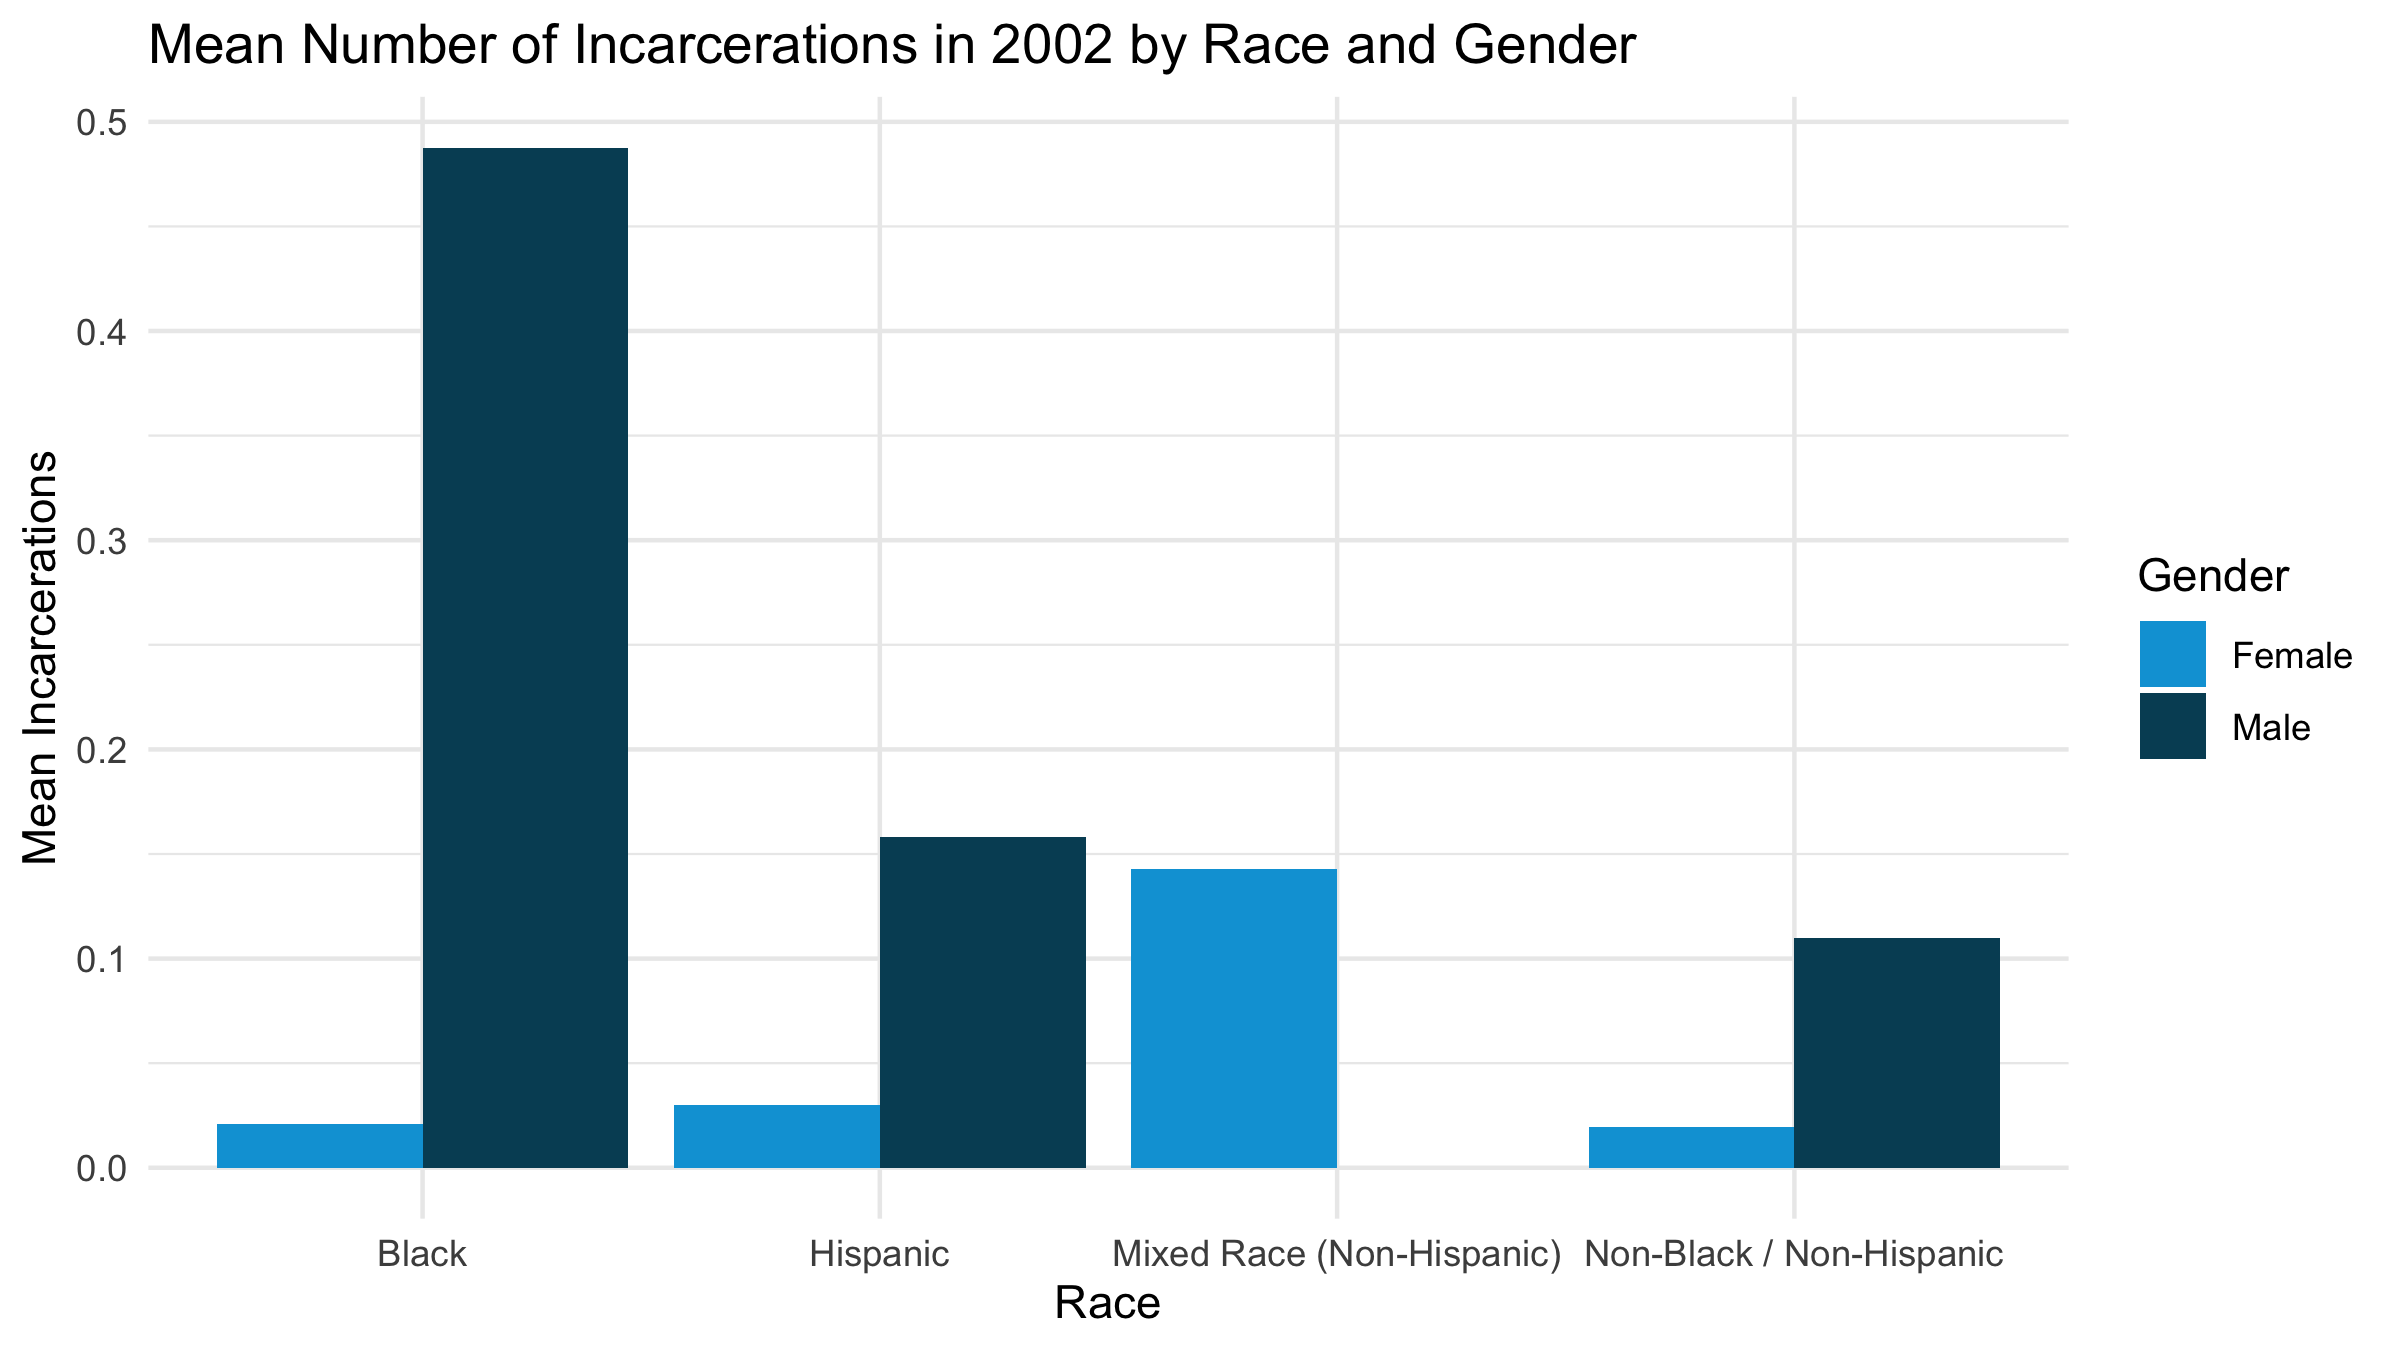
\includegraphics[width=.85\textwidth]{incarcerations_by_racegender}
    \end{center}
    \caption{Mean Number of Incarcerations in 2002 by Race and Gender (this is the LaTeX caption, not the ggplot title)}
    \label{fig:graph}
\end{figure}

The Figure \ref{fig:graph} above is a barplot showing the mean number of incarcerations in 2002 by \texttt{race} and \texttt{gender}.

For respondents whose variable \texttt{race} is \texttt{Black}, 


\begin{table}[H]

\caption{\label{tab:tab:summarystats}Mean Number of incarcerated Months in 2002 by Race and Gender}
\centering
\begin{tabular}[t]{lrrrr}
\toprule
Gender & Black & Hispanic & Mixed Race Non Hispanic & Non Black Non Hispanic\\
\midrule
\cellcolor{gray!6}{Female} & \cellcolor{gray!6}{0.0211268} & \cellcolor{gray!6}{0.0298013} & \cellcolor{gray!6}{0.1428571} & \cellcolor{gray!6}{0.0193192}\\
Male & 0.4876712 & 0.1579509 & 0.0000000 & 0.1099476\\
\bottomrule
\end{tabular}
\end{table}



% Table created by stargazer v.5.2.2 by Marek Hlavac, Harvard University. E-mail: hlavac at fas.harvard.edu
% Date and time: Thu, Feb 17, 2022 - 02:37:03
\begin{table}[!htbp] \centering 
  \caption{Regression Output. Omitted category is Black Females.} 
  \label{tab:regression} 
\begin{tabular}{@{\extracolsep{5pt}}lc} 
\\[-1.8ex]\hline 
\hline \\[-1.8ex] 
 & \multicolumn{1}{c}{\textit{Dependent variable:}} \\ 
\cline{2-2} 
\\[-1.8ex] & Incarcerations in 2002 \\ 
\hline \\[-1.8ex] 
 Hispanic & $-$0.159$^{***}$ \\ 
  & (0.038) \\ 
  & \\ 
 Mixed Race (Non-Hispanic) & $-$0.174$^{**}$ \\ 
  & (0.083) \\ 
  & \\ 
 Non-Black / Non-Hispanic & $-$0.189$^{***}$ \\ 
  & (0.035) \\ 
  & \\ 
 Male & 0.194$^{***}$ \\ 
  & (0.022) \\ 
  & \\ 
 Constant & 0.155$^{***}$ \\ 
  & (0.026) \\ 
  & \\ 
\hline \\[-1.8ex] 
Observations & 8,621 \\ 
R$^{2}$ & 0.015 \\ 
Adjusted R$^{2}$ & 0.014 \\ 
Residual Std. Error & 1.019 (df = 8616) \\ 
F Statistic & 32.033$^{***}$ (df = 4; 8616) \\ 
\hline 
\hline \\[-1.8ex] 
\textit{Note:}  & \multicolumn{1}{r}{$^{*}$p$<$0.1; $^{**}$p$<$0.05; $^{***}$p$<$0.01} \\ 
\end{tabular} 
\end{table} 


\section{The Next Steps}

\end{document}
